\documentclass[a4paper,11pt,fleqn]{article}%fleqn pour aligner les equations à gauche
\usepackage{../../Styles/Cours}


\newcommand{\chnum}{Chapitre 16}
\newcommand{\chtitle}{Rendement d'une cellule photoélectrique}
\newcommand{\dtype}{TP}

\begin{document}
	\maketitle
Les cellules photovoltaïques dont des dispositifs de plus en plus utilisés aujourd'hui. En effet, elles ont l'avantage de produire de l'électricité à partir d'une source d'énergie abondante : le rayonnement solaire. comment déterminer le rendement d'une cellule photovoltaïque ?

\begin{figure}[h!]
	\subfloat[Protocole et montage]{
	\begin{minipage}{.5\linewidth}
	\centering \begin{circuitikz}
        %\draw[gray!10] (0,0) grid (6,6);
        \draw (0,0) 
        to [pvsource, i^>=$i$, mirror] (0,3)
        to [short] (0,3)
        to [short] (2,3)
        to [rmeter, t=V, v=$U$] (2,0)
        to [short] (2,0)
        to (0,0)
        ;
        \draw (2,3)
        to [rmeter, t=A] (5,3)
        to [vR, invert] (5,0)
        to (2,0)
        ;
    \end{circuitikz}
    
    \begin{itemize}
    		\item[-] Éclairer la cellule de manière à ce que les rayons arrivent perpendiculairement par rapport à la cellule.
    		\item[-] Faire varier la résistance du résistor au moins dix fois et, pour chacune de ces valeurs mesurer l'intensité du courant ainsi que la tension aux bornes de la cellule.
    		\item[-] Pour chaque couple ($U$, $I$), calculer la puissance électrique.
    	\end{itemize}
    	\label{fig1}
    	\end{minipage}
    }
    \subfloat[Caractéristiques d'une cellule]{
    \begin{minipage}{.5\linewidth}
    \centering 	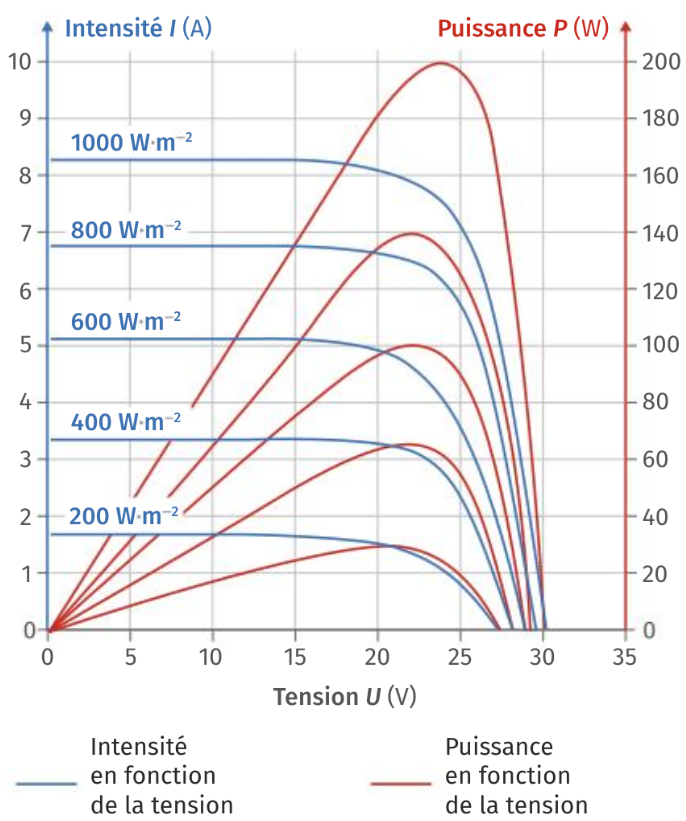
\includegraphics[width=.8\linewidth]{Ressources/TSPE_C16_Act2_fig2.png}
    	\end{minipage}
    	\label{fig2}
    	}
\end{figure}

\noindent \colorbox{blue!10}{
    \begin{minipage}{.98\linewidth}
    \centering  \textcolor{purple!50!blue!70}{\Large \textbf{Questions}}
    \begin{enumerate}
        \item Représenter la chaîne énergétique du panneau photovoltaïque, en identifiant les puissances reçues, perdues et utiles, et en nommant la forme d'énergie associée.
        \item Commenter les courbes du \ref{fig2}.
        \item Tracer la caractéristique $I=f(U)$, puis la courbe $P=f(U)$ de la cellule. Déterminer la puissance maximale de la cellule, appelée puissance de crête.
        \item Avec le  luxmètre, mesurer la puissance surfacique reçue par la cellule. En déduire le rendement du panneau.
        \item Proposer et mettre en \oe uvre un protocole permettant de tracer l'évolution du rendement de la cellule en fonction de l'angle d'incidence des rayons lumineux.
        \item Lister les paramètres influençant le rendement d'une cellule photovoltaïque.
    \end{enumerate}
    \end{minipage}
}
\end{document}
